\subsection{Vue}

% https://www.w3schools.com/vue/
% https://developer.mozilla.org/en-US/docs/Learn/Tools_and_testing/Client-side_JavaScript_frameworks/Vue_getting_started
% https://www.tutorialspoint.com/vuejs/vuejs_overview.htm
% https://www.itnetwork.cz/javascript/vuejs/uvod-do-vuejs-a-prvni-aplikace
% https://worldline.github.io/vuejs-training/
% https://www.rascasone.com/cs/blog/co-je-framework-vuejs

Vue dostalo svůj název díky anglickému slovu view. Jedná se o~deklarativní JavaScriptový open-source framework. 
Je určen k~efektivní tvorbě jak jednoduchých, tak i~komplexních uživatelských rozhraní na webu. 
Framework je v~současné době jedním z~nejpopulárnějších frameworků pro tvorbu webových aplikací.\cite{vuemacrae,vue}

\begin{figure}[htb]
	\centering
		
\includegraphics[width=.3\textwidth]{images/vue-logo.png}
	\caption[Vue logo]{Vue logo \cite{vue}}
	\label{fig:vuelogo}
\end{figure}

Evan You, tvůrce Vue.js, se inspiroval určitými částmi frameworku AngularJS, který však měl velmi strmou křivku učení. 
Vue tedy mělo být lehké, přizpůsobivé a~snadné k~naučení. Bylo vytvořeno roku~2013, uvolněno do světa až o~rok později. 
Od té doby byly vydány pouze 3 majoritní verze, avšak ty přinesly mnoho změn.\cite{vueflexiple,vuemedium}

Vue nabízí svobodnou volbu při tvorbě komponent ve formě dvou hlavních API -- Options a~Composition API. 
Options API můžeme přirovnat k~objektovému přístupu, kdežto Composition API využívá funkcionální přístup. 
Podle \cite{vue} Composition API přináší větší flexibilitu a~umožňuje efektivnější návrhové vzory pro organizaci a~znovupoužitelnost kódu. 
Z~tohoto důvodu v~analýze budeme využívat Composition API.

Framework klade důraz na progresivitu, což znamená, že roste s~vývojářem a~přizpůsobuje se jeho potřebám. 
Díky tomu si Vue oblíbily společnosti jako Xiaomi, Adobe, Gitlab, Trivago, BMW.\cite{vuetriodev,vue}

\subsubsection{Single-File Components}

Základní funkcí Vue jsou tzv. Single-File Components (SFC). Jedná se o~hlavní stavební blok frameworku, který reprezenzuje část webové stránky. 
Komponenta se skládá ze šablony, dat komponenty, funkcí a~kaskádových stylů. Hlavní výhodu tohoto přístupu představuje znovupoužitelnost. 
JavaScriptové funkce musí být zapsány mezi párové značky script s~atributem setup, šablona do template tagů a~styly do style bloku.\cite{vuemacrae,vue}

\begin{prog}
<script setup>
  import \{ ref \} from 'vue';
  
  const content = ref('nějaký-obsah');
</script>
  
<template>
  <div>\{\{ content \}\}</div>
</template>
  
<style scoped>
  div \{
    background-color: red;
  \}
</style>
\end{prog}

\subsubsection{Reaktivita}

V~komponentě můžeme uchovávat informace pomocí reaktivních stavů. Oficiální dokumentace doporučuje používat funkci ref, která vyžaduje počáteční hodnotu. 
K~hodnotě stavu pak v~rámci skriptu přistupujeme pomocí vlastnosti value. V~šabloně postačí pouze název stavu. 
Modifikaci stavu lze provést pomocí přiřazení nové hodnoty. Při změně jakéhokoli stavu komponenty pak Vue automaticky aktualizuje DOM novými daty.\cite{vue}

\begin{prog}
<script setup>
  import \{ ref \} from 'vue';
  
  const count = ref(0);

  function increment() \{
    count.value++;
  \}
</script>
  
<template>
  <button v-on:click="increment">
    Klikli jste na tlačítko \{\{ count \}\}x.
  </button>
</template>
\end{prog}

\subsubsection{Předávání vlastností}

Komponenty spolu komunikují pomocí předávání vlastností. 
Pro předání vlastnosti do vnořené komponenty je třeba v~rodičovské komponentě předat požadovanou hodnotu do proměnné vnořené komponenty. 
Uvnitř vnořené komponenty pak definujeme props vlastnost, kterou vytvoříme pomocí funkce defineProps. 
DefineProps funkce vyžaduje objekt s~názvem a~datovým typem předávané vlastnosti.

K~předání vlastností z~vnořené do rodičovské komponenty se využívá principu emitování eventů. 
V~potomku vytvoříme vlastnost emit, v~níž nadeklarujeme pole emitovaných hodnot pomocí funkce defineEmits. Dále je třeba definovat jednotlivé emity. 
Prvním argumentem je název emitu, další argumenty jsou již předávané hodnoty. Rodičovská komponenta musí naslouchat na emitované eventy. 
Toho lze docílit pomocí @response direktivy, která typicky v~callback funkci přeukládá argumenty na lokalní stavy.\cite{vuemacrae,vue}

% TODO: přidat příklad s emitováním eventu
% <script setup>
% import { ref } from 'vue'
% import ChildComponent from './Comp.vue'

% const msg = ref('Hello World!')

% function handleChildSubmit(data) {
%  console.log(data.message) // Outputs: "Form submitted!"
% }
% </script>

% <template>
%   <h1>{{ msg }}</h1>
%   <input v-model="msg" />

%   <ChildComponent @submit="handleChildSubmit" />
% </template>


% <script setup>
%   const emit = defineEmits(['submit'])
  
%   function handleSubmit() {
%   // Emit the 'submit' event with some data
%     emit('submit', { message: 'Form submitted!' })
%   }
% </script>

% <template>
%   <button @click="handleSubmit">Submit</button>
% </template>

\begin{prog}
// Parent.vue
<script setup>
  import \{ ref \} from 'vue';
  import ChildComponent from './Child.vue';

  const someProps = ref(\{color: 'cervena'\});
</script>

<template>
	<ChildComponent :color="'cervena'" />
  <ChildComponent :color="someProps.color" />
</template>

// Child.vue
<script setup>
  const props = defineProps(\{
    color: String
  \});
</script>

<template>
  <div :class="color"></div>
</template>
\end{prog}

\subsubsection{Direktivy a eventy}

Framework disponuje mnoha direktivami, které umožňují přidávat do šablony různé funkce. Logiku vykreslování umožňují direktivy v-if, v-else-if a~v-else. 
Pro iteraci přes pole hodnot slouží v-for. Mezi další užitečné direktivy patří v-bind a~v-model. 
Díky v-bind je možné přidat jakémukoli elementu dynamickou hodnotu atributu, direktivu můžeme zkrátit pomocí dvojtečky. 
Direktiva v-model zase zajistí obousměrné propojení pro formulářové prvky.

\begin{prog}
<script setup>
  import \{ ref \} from 'vue';

  const text = ref('');
</script>

<template>
  <input v-model="text" placeholder="Něco napište">
  <p v-if="text.length > 3">\{\{ text \}\}</p>
  <p v-else>Musíte zadat více než 3 znaky</p>
</template> 
\end{prog}

Vue také umožnuje naslouchat na DOM eventy pomocí direktivy v-on. Ta pak vyžaduje libovolný DOM event a~callback funkci, jež se vykoná při daném DOM eventu. 
Můžeme také zvolit ekvivalentní zápis s~@. Další možnost představuje využití modifkátorů eventů, které se postarají například o~vypnutí výchozího chování prvku.\cite{vuemacrae,vue}

\begin{prog}
<script setup>
  import \{ ref \} from 'vue';

  const count = ref(0);
</script>

<template>
  <button @click="() => count++">
    Klikli jste na tlačítko \{\{ count \}\}x.
  </button>
</template>
\end{prog}

\subsubsection{Životní cyklus}

Každá Vue komponenta má daný životní cyklus, který konkrétně můžeme rozdělit na 3~části -- inicializační část, část, při které se mění data a~část, kdy komponenta zaniká. 
Pro zajištění kontroly životního cyklu slouží tzv. hooks, které se vyznačují tím, že vždy před svým názvem mají předponu on.

\begin{figure}[htb]
	\centering
		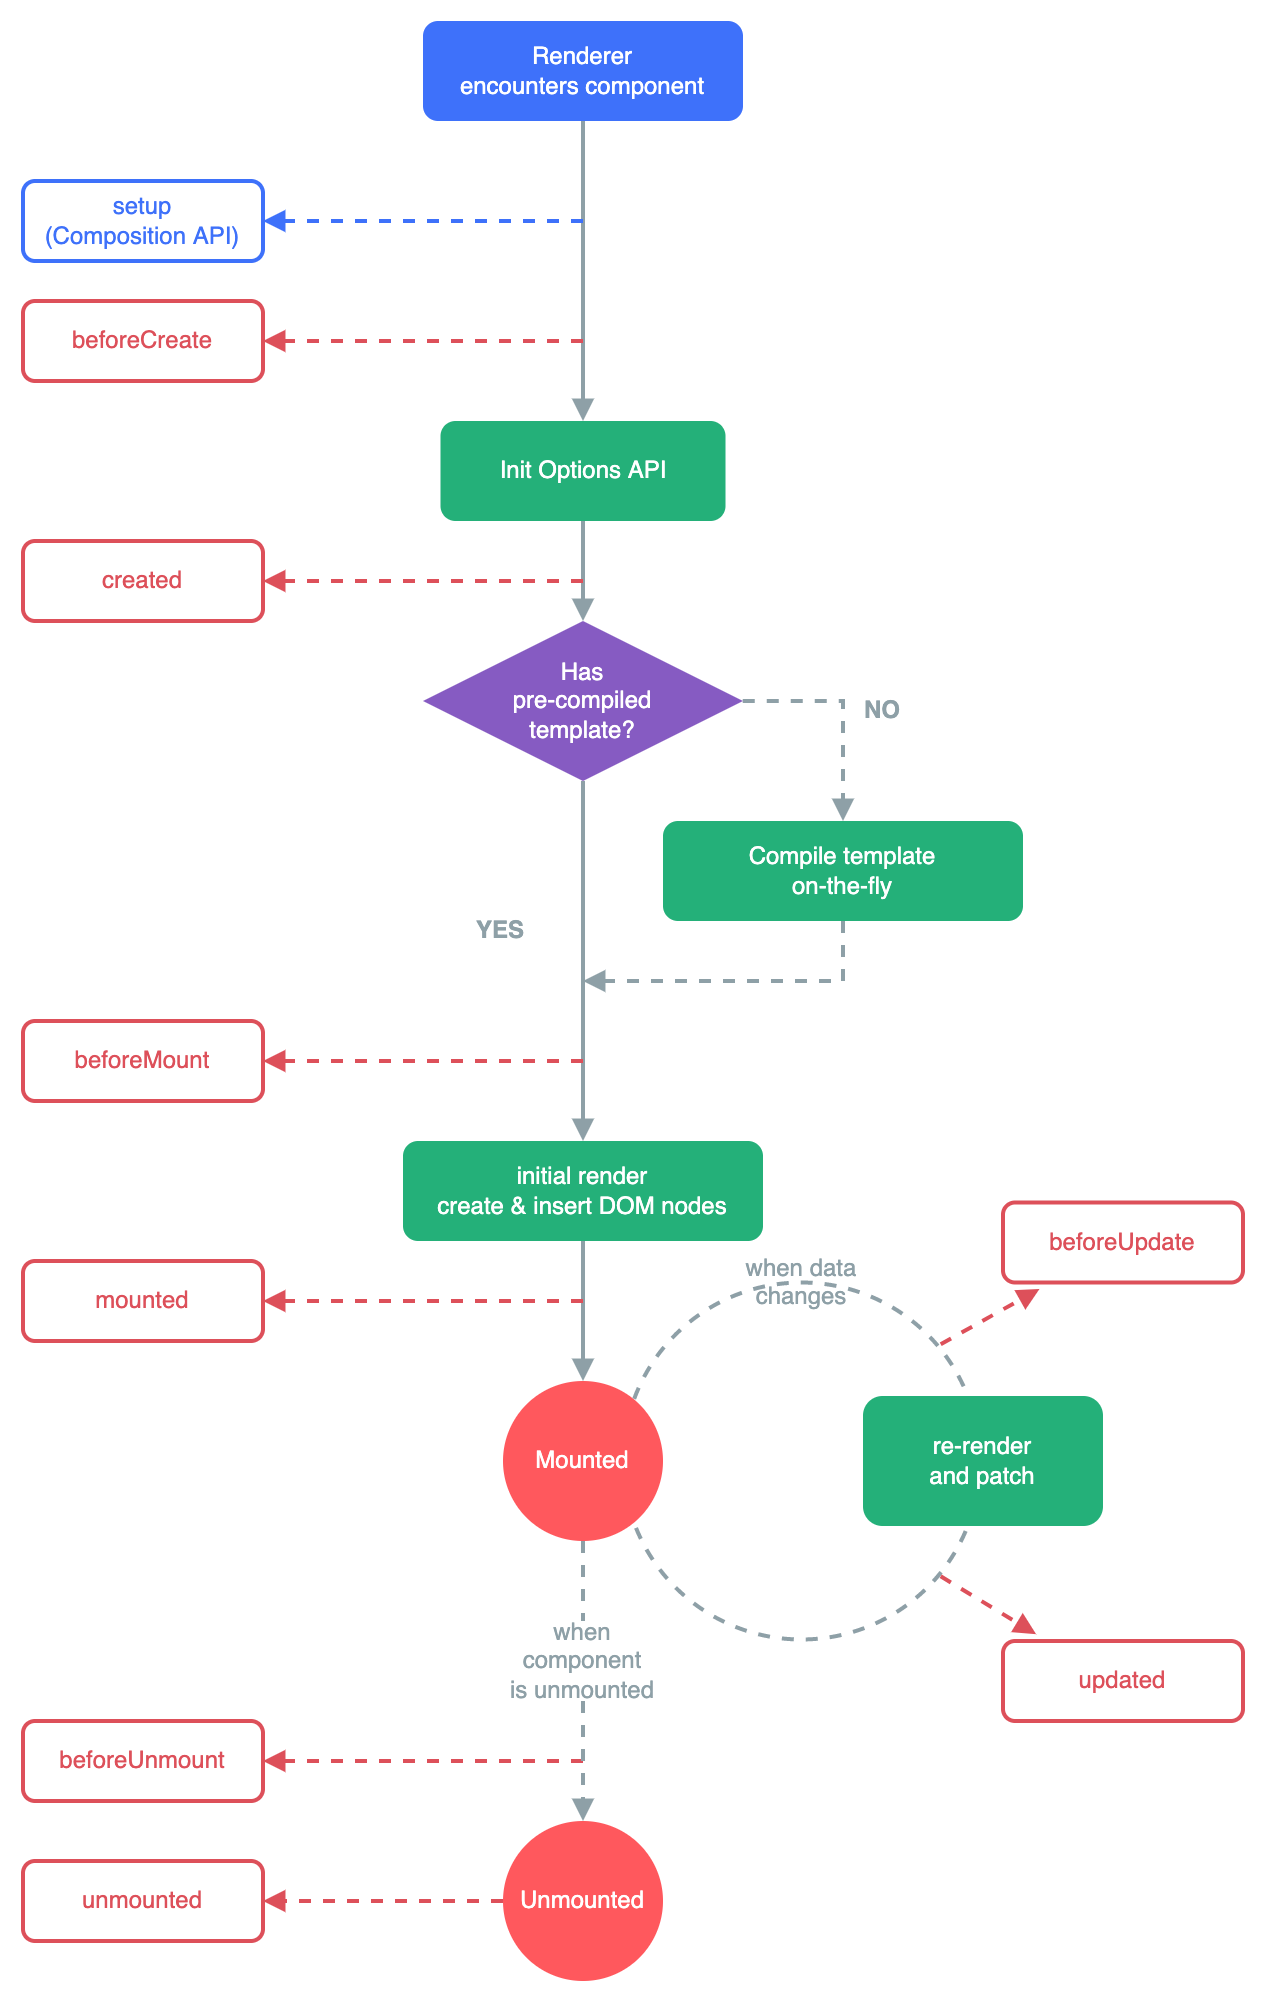
\includegraphics[width=.7\textwidth]{images/vuelifecycle.png}
	\caption[Životní cyklus Vue komponenty]{Životní cyklus Vue komponenty \cite{vue}}
	\label{fig:vuelifecycle}
\end{figure}

Při inicializaci komponenty můžeme využít hook akce beforeMount či mount. BeforeMount je volán ještě před tím, než se komponenta přidá na stránku. 
Mount až poté, kdy je vytvořen element komponenty -- komponenta však ještě nemusí být v~DOM. 
Před chystanou změnou dat v~DOM se volá beforeUpdate, po vykonání změny je volán hook updated. Před samotným zánikem komponenty pak Vue volá beforeUnmount. 
Po dokončení zničení se volá hook unmounted.\cite{vuemacrae,vue}

\subsubsection{State management}

Framework Vue v~sobě nemá implementovaný žádný sofistikovaný state management. 
K~základní práci se stavy aplikace poslouží reaktivní stavy jednotlivých komponent a~jejich sdílení ve stromě komponent.

Pro komplexnější aplikace je žádoucí využít některou z~knihoven třetích stran. Dokumentace nabízí knihovnu Pinia, která byla vyvinuta Vue týmem. 
Pinia je inspirována balíkem Vuex a~využívá Composition API přístup. Knihovna nabízí jednoduché API pro správu stavů aplikace. 
Hlavním prvkem jsou tzv.~stores, do kterých ukládáme globální stavy aplikace. 
Store vytvoříme pomocí funkce defineStore, která požaduje identifikátor daného store a~callback funkci. 
Ta by měla vracet samotný state definovaný pomocí ref() a~akce (funkce, jež mění stavy) nad storem, případně computed state -- jiný stav, který je typicky odvozen od původního stavu.\cite{pinia,vue}

\subsubsection{Routování}

Samotný Vue framework neposkytuje zabudovanou podporu pro routování. Oficiální dokumentace doporučuje využití knihovny Vue Router, která umožňuje routování na straně klienta. 
Základní využití routeru spočívá ve vytvoření instance routeru. Tuto instanci inicializujeme polem požadovaných cest aplikace s~konkrétními komponentami pro vykreslení. 
V~rámci šablony pak můžeme použít router-link element, jež představuje odkaz na jinou cestu. Pro vykreslení obsahu po změně cesty slouží router-view. 
V~podstatě se jedná o~wrapper pro vykreslení komponenty, která je spojena s~uživatelem vybranou cestou.

Vue Router disponuje také dynamickým routingem, který umožňuje definovat parametry cesty a~vykreslit tedy stránku s~dynamickými daty. 
Mezi další funkce patří např.~zanořené routování a~routování dle pojmenovaných cest aplikace.\cite{vue,vuerouter}

\subsubsection{Ekosystém}

Vue framework sice nabízí solidní základ pro vývoj webových aplikací, sám o~sobě ale není komplexním nástrojem pro vývoj aplikací většího rozsahu. 
Většina vývojářů využívá kromě frameworku i~další knihovny třetích stran, které zvyšují produktivitu a~zjednodušují vývoj požadovaných funkcí. 
V~rámci ekosystému lze využít například knihovny pro práci s~UI komponenty, routováním, state managementem. 
Nechybí ani knihovny pro typování, testování, statické generování či formátování kódu.

Při rostoucí komplexitě webových aplikací můžeme zvážit použití pokročilého frameworku Nuxt. Nuxt je postaven na základech Vue.js a~poskytuje production-ready nástroje. 
Konkrétně řeší například pokročilou správu stavů, routing, hydrataci stránek či Server Side Rendering.\cite{awesomevue,vue}